% This file was created with matplot2tikz v0.5.4.
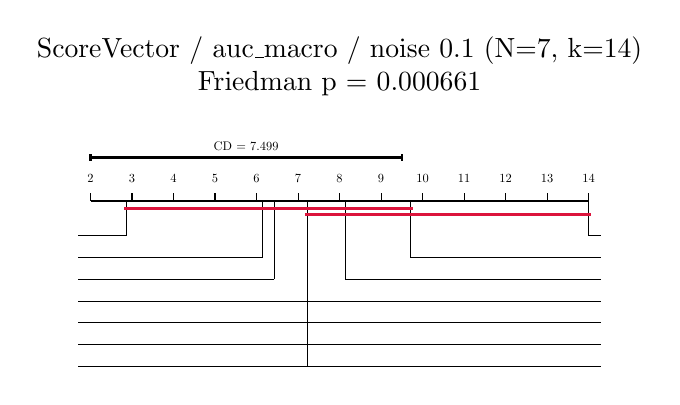
\begin{tikzpicture}

\definecolor{crimson}{RGB}{220,20,60}
\definecolor{darkgray176}{RGB}{176,176,176}

\begin{axis}[
hide x axis,
hide y axis,
tick align=outside,
tick pos=left,
title style={align=center},
title={ScoreVector / auc\_macro / noise 0.1  (N=7, k=14)\\Friedman p = 0.000661},
x grid style={darkgray176},
xmin=1.5, xmax=14.5,
xtick style={color=black},
y grid style={darkgray176},
ymin=-8.5, ymax=1.8,
ytick style={color=black}
]
\addplot [black]
table {%
2 0
14 0
};
\addplot [black]
table {%
2 0
2 0.18
};
\addplot [black]
table {%
3 0
3 0.18
};
\addplot [black]
table {%
4 0
4 0.18
};
\addplot [black]
table {%
5 0
5 0.18
};
\addplot [black]
table {%
6 0
6 0.18
};
\addplot [black]
table {%
7 0
7 0.18
};
\addplot [black]
table {%
8 0
8 0.18
};
\addplot [black]
table {%
9 0
9 0.18
};
\addplot [black]
table {%
10 0
10 0.18
};
\addplot [black]
table {%
11 0
11 0.18
};
\addplot [black]
table {%
12 0
12 0.18
};
\addplot [black]
table {%
13 0
13 0.18
};
\addplot [black]
table {%
14 0
14 0.18
};
\addplot [line width=0.32pt, black]
table {%
2.85714285714286 0
2.85714285714286 -0.8
};
\addplot [line width=0.32pt, black]
table {%
2.85714285714286 -0.8
1.7 -0.8
};
\addplot [line width=0.32pt, black]
table {%
6.14285714285714 0
6.14285714285714 -1.3
};
\addplot [line width=0.32pt, black]
table {%
6.14285714285714 -1.3
1.7 -1.3
};
\addplot [line width=0.32pt, black]
table {%
6.42857142857143 0
6.42857142857143 -1.8
};
\addplot [line width=0.32pt, black]
table {%
6.42857142857143 -1.8
1.7 -1.8
};
\addplot [line width=0.32pt, black]
table {%
7.21428571428571 0
7.21428571428571 -2.3
};
\addplot [line width=0.32pt, black]
table {%
7.21428571428571 -2.3
1.7 -2.3
};
\addplot [line width=0.32pt, black]
table {%
7.21428571428571 0
7.21428571428571 -2.8
};
\addplot [line width=0.32pt, black]
table {%
7.21428571428571 -2.8
1.7 -2.8
};
\addplot [line width=0.32pt, black]
table {%
7.21428571428571 0
7.21428571428571 -3.3
};
\addplot [line width=0.32pt, black]
table {%
7.21428571428571 -3.3
1.7 -3.3
};
\addplot [line width=0.32pt, black]
table {%
7.21428571428571 0
7.21428571428571 -3.8
};
\addplot [line width=0.32pt, black]
table {%
7.21428571428571 -3.8
1.7 -3.8
};
\addplot [line width=0.32pt, black]
table {%
7.21428571428571 0
7.21428571428571 -3.8
};
\addplot [line width=0.32pt, black]
table {%
7.21428571428571 -3.8
14.3 -3.8
};
\addplot [line width=0.32pt, black]
table {%
7.21428571428571 0
7.21428571428571 -3.3
};
\addplot [line width=0.32pt, black]
table {%
7.21428571428571 -3.3
14.3 -3.3
};
\addplot [line width=0.32pt, black]
table {%
7.21428571428571 0
7.21428571428571 -2.8
};
\addplot [line width=0.32pt, black]
table {%
7.21428571428571 -2.8
14.3 -2.8
};
\addplot [line width=0.32pt, black]
table {%
7.21428571428571 0
7.21428571428571 -2.3
};
\addplot [line width=0.32pt, black]
table {%
7.21428571428571 -2.3
14.3 -2.3
};
\addplot [line width=0.32pt, black]
table {%
8.14285714285714 0
8.14285714285714 -1.8
};
\addplot [line width=0.32pt, black]
table {%
8.14285714285714 -1.8
14.3 -1.8
};
\addplot [line width=0.32pt, black]
table {%
9.71428571428571 0
9.71428571428571 -1.3
};
\addplot [line width=0.32pt, black]
table {%
9.71428571428571 -1.3
14.3 -1.3
};
\addplot [line width=0.32pt, black]
table {%
14 0
14 -0.8
};
\addplot [line width=0.32pt, black]
table {%
14 -0.8
14.3 -0.8
};
\addplot [thick, black]
table {%
2 1
9.49891726369177 1
};
\addplot [thick, black]
table {%
2 0.92
2 1.08
};
\addplot [thick, black]
table {%
9.49891726369177 0.92
9.49891726369177 1.08
};
\addplot [very thick, crimson]
table {%
2.80714285714286 -0.18
9.76428571428571 -0.18
};
\addplot [very thick, crimson]
table {%
7.16428571428571 -0.31
14.05 -0.31
};
\draw (axis cs:2,0.32) node[
  scale=0.45,
  anchor=south,
  text=black,
  rotate=0.0
]{2};
\draw (axis cs:3,0.32) node[
  scale=0.45,
  anchor=south,
  text=black,
  rotate=0.0
]{3};
\draw (axis cs:4,0.32) node[
  scale=0.45,
  anchor=south,
  text=black,
  rotate=0.0
]{4};
\draw (axis cs:5,0.32) node[
  scale=0.45,
  anchor=south,
  text=black,
  rotate=0.0
]{5};
\draw (axis cs:6,0.32) node[
  scale=0.45,
  anchor=south,
  text=black,
  rotate=0.0
]{6};
\draw (axis cs:7,0.32) node[
  scale=0.45,
  anchor=south,
  text=black,
  rotate=0.0
]{7};
\draw (axis cs:8,0.32) node[
  scale=0.45,
  anchor=south,
  text=black,
  rotate=0.0
]{8};
\draw (axis cs:9,0.32) node[
  scale=0.45,
  anchor=south,
  text=black,
  rotate=0.0
]{9};
\draw (axis cs:10,0.32) node[
  scale=0.45,
  anchor=south,
  text=black,
  rotate=0.0
]{10};
\draw (axis cs:11,0.32) node[
  scale=0.45,
  anchor=south,
  text=black,
  rotate=0.0
]{11};
\draw (axis cs:12,0.32) node[
  scale=0.45,
  anchor=south,
  text=black,
  rotate=0.0
]{12};
\draw (axis cs:13,0.32) node[
  scale=0.45,
  anchor=south,
  text=black,
  rotate=0.0
]{13};
\draw (axis cs:14,0.32) node[
  scale=0.45,
  anchor=south,
  text=black,
  rotate=0.0
]{14};
\draw (axis cs:1.6,-0.8) node[
  scale=0.45,
  anchor=east,
  text=black,
  rotate=0.0
]{CLR  (2.86)};
\draw (axis cs:1.6,-1.3) node[
  scale=0.45,
  anchor=east,
  text=black,
  rotate=0.0
]{ECC  (6.14)};
\draw (axis cs:1.6,-1.8) node[
  scale=0.45,
  anchor=east,
  text=black,
  rotate=0.0
]{LP  (6.43)};
\draw (axis cs:1.6,-2.3) node[
  scale=0.45,
  anchor=east,
  text=black,
  rotate=0.0
]{IA6  (7.21)};
\draw (axis cs:1.6,-2.8) node[
  scale=0.45,
  anchor=east,
  text=black,
  rotate=0.0
]{IA2  (7.21)};
\draw (axis cs:1.6,-3.3) node[
  scale=0.45,
  anchor=east,
  text=black,
  rotate=0.0
]{IA5  (7.21)};
\draw (axis cs:1.6,-3.8) node[
  scale=0.45,
  anchor=east,
  text=black,
  rotate=0.0
]{IA8  (7.21)};
\draw (axis cs:14.4,-3.8) node[
  scale=0.45,
  anchor=west,
  text=black,
  rotate=0.0
]{(7.21)  IA7};
\draw (axis cs:14.4,-3.3) node[
  scale=0.45,
  anchor=west,
  text=black,
  rotate=0.0
]{(7.21)  IA3};
\draw (axis cs:14.4,-2.8) node[
  scale=0.45,
  anchor=west,
  text=black,
  rotate=0.0
]{(7.21)  IA4};
\draw (axis cs:14.4,-2.3) node[
  scale=0.45,
  anchor=west,
  text=black,
  rotate=0.0
]{(7.21)  IA1};
\draw (axis cs:14.4,-1.8) node[
  scale=0.45,
  anchor=west,
  text=black,
  rotate=0.0
]{(8.14)  CC};
\draw (axis cs:14.4,-1.3) node[
  scale=0.45,
  anchor=west,
  text=black,
  rotate=0.0
]{(9.71)  BR};
\draw (axis cs:14.4,-0.8) node[
  scale=0.45,
  anchor=west,
  text=black,
  rotate=0.0
]{(14.00)  MLkNN};
\draw (axis cs:5.74945863184589,1.15) node[
  scale=0.45,
  anchor=base,
  text=black,
  rotate=0.0
]{CD = 7.499};
\end{axis}

\end{tikzpicture}
